\documentclass[12pt]{article}

% Packages
\usepackage[utf8]{inputenc}
\usepackage{amsmath}
\usepackage{amssymb}
\usepackage{graphicx}
\usepackage{hyperref}
\usepackage{amsthm}
\usepackage[margin=1in]{geometry}
\usepackage[numbers]{natbib}
\usepackage{listings}
\usepackage{algorithm}
\usepackage{algpseudocode}
\usepackage{tabularx}

% TikZ and diagram packages
\usepackage{tikz}
\usetikzlibrary{positioning,arrows,shapes,calc,decorations.pathreplacing}
\usepackage{forest}

% Theorem environments
\newtheorem{theorem}{Theorem}
\newtheorem{lemma}{Lemma}
\newtheorem{proposition}{Proposition}
\newtheorem{corollary}{Corollary}
\newtheorem{hypothesis}{Hypothesis}
\newtheorem{definition}{Definition}
\newtheorem{remark}{Remark}
\newtheorem{constraint}{Constraint}

% Title and author
\title{A Template for Transforming Raw Text into Structured Academic Discourse}
\author{Author Name}
\date{\today}

\begin{document}
\maketitle
\begin{abstract}
This paper presents a generic research-style exposition that can serve as a template when transforming unstructured input text into a structured academic paper. In the absence of specific domain content, the discussion focuses on the methodology of such transformations: how to identify latent research questions, impose a conventional scholarly structure, and enrich the resulting document with formal elements such as definitions, theorems, diagrams, and tables. The paper outlines a conceptual workflow, proposes a simple theoretical model of text transformation, and illustrates how logical organization and incremental refinement can turn informal material into a coherent research narrative. The aim is to offer a reusable pattern that can be instantiated once concrete source content is available.
\end{abstract}

\section{Introduction}

Transforming raw or informal text into a structured academic paper is a common yet under-theorized task, even in areas where large-scale datasets and models have been introduced to study research article generation from heterogeneous project materials \cite{ref_1}. In many workflows, researchers, editors, and automated systems must convert heterogeneous materials—notes, reports, or incomplete drafts—into documents that follow recognized scholarly conventions. This paper proposes a generic framework for such transformations in settings where the target is an academic research paper but the initial content is incomplete or underspecified.

The discussion abstracts away from any specific scientific domain and concentrates instead on structure and method. The central idea is that any sufficiently rich input text can be reorganized along three axes:
\begin{itemize}
  \item a \emph{conceptual axis}, which identifies the core problem, claims, and contributions;
  \item a \emph{structural axis}, which organizes content into sections and subsections obeying academic norms;
  \item a \emph{formal axis}, which expresses key ideas as definitions, equations, or theorems when appropriate.
\end{itemize}

The remainder of this template-like paper illustrates how one might proceed when the source content is absent or minimal. Rather than fabricating domain-specific facts, the paper focuses on outlining a generic, reusable methodology that can complement data-driven approaches to article generation \cite{ref_1} by making the underlying structural and conceptual decisions explicit.

\section{Background and Motivation}

Academic writing is governed by conventions that support clarity, reproducibility, and critical evaluation \cite{ref_2}. These conventions typically include an abstract, an introduction, a review of relevant context, a description of methods, an analysis of results, and a discussion of implications, often instantiated in practice through the widely adopted IMRAD (Introduction, Methods, Results, and Discussion) structure \cite{ref_3}. When the starting point is unstructured text, these components are often implicit rather than explicit, and the rhetorical moves that signal them may be only partially realized.

Motivating scenarios include:
\begin{itemize}
  \item Draft notes from collaborative meetings that need to be turned into a paper.
  \item Technical reports or documentation that must be reframed as research articles.
  \item Informal descriptions generated by automated systems that require scholarly refinement, including systems trained on project data to produce article bodies \cite{ref_1}.
\end{itemize}

In such settings, the challenge is not only to rephrase the text but to make explicit a research narrative: an identifiable problem, a method, a result, and a contribution. Genre-based models of research writing, such as CARS (Create a Research Space), emphasize how introductions and other sections encode these moves in systematic ways \cite{ref_2,ref_3}. This paper treats the problem at a meta-level, characterizing the transformation process itself as an object of study and providing a template that can be aligned with established genre structures.

\section{Conceptual Framework for Text Transformation}

\subsection*{Abstract mapping from input text to structured paper}
Introduces the core mathematical representation of the transformation from raw text to academic paper and its compositional decomposition, aligning with genre-aware structuring stages such as IMRAD and CARS.

\begin{align*}
F : \mathcal{T} &\to \mathcal{P}, \\
F &= F_{\mathrm{formal}} \circ F_{\mathrm{struct}} \circ F_{\mathrm{concept}}.
\end{align*}

To reason about transforming input text into a research paper, it is helpful to introduce a simple abstract model. Let $T$ denote an input text artifact and $P$ a structured paper. We can think of the transformation as a mapping
\begin{equation*}
  F : \mathcal{T} \to \mathcal{P},
\end{equation*}
where $\mathcal{T}$ is the space of possible unstructured texts and $\mathcal{P}$ the space of structured academic papers.

We conceptually decompose $F$ into three stages:
\begin{equation*}
  F = F_{\mathrm{formal}} \circ F_{\mathrm{struct}} \circ F_{\mathrm{concept}},
\end{equation*}
where
\begin{itemize}
  \item $F_{\mathrm{concept}}$ extracts and clarifies the central ideas, questions, and claims.
  \item $F_{\mathrm{struct}}$ maps these ideas into a canonical paper organization, such as IMRAD or related variants \cite{ref_3}.
  \item $F_{\mathrm{formal}}$ enriches the paper with formal elements (definitions, equations, diagrams) as appropriate.
\end{itemize}

This compositional perspective emphasizes that successful transformation is not a single monolithic operation but an iterative process of conceptual clarification, structural alignment with disciplinary genres \cite{ref_2,ref_3}, and formal refinement. It is compatible with data-driven pipelines that learn such mappings from large corpora \cite{ref_1}, while making the intermediate representational stages explicit.

\section{Methodology for Structuring Academic Content}

\subsection*{Pipeline for transforming input text into a research paper}
A simple TikZ diagram illustrating the three-stage pipeline from raw text to structured academic paper, with an intermediate structural stage that can encode conventions such as IMRAD or CARS.

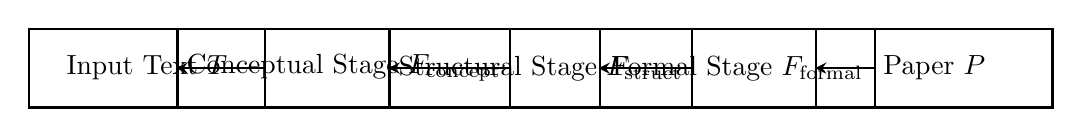
\begin{tikzpicture}[node distance=2.5cm,>=stealth,thick]
  \node[draw, rectangle, minimum width=3cm, minimum height=1cm] (input) {Input Text $T$};
  \node[draw, rectangle, minimum width=3.5cm, minimum height=1cm, right of=input] (concept) {Conceptual Stage $F_{\mathrm{concept}}$};
  \node[draw, rectangle, minimum width=3.5cm, minimum height=1cm, right of=concept] (struct) {Structural Stage $F_{\mathrm{struct}}$};
  \node[draw, rectangle, minimum width=3.5cm, minimum height=1cm, right of=struct] (formal) {Formal Stage $F_{\mathrm{formal}}$};
  \node[draw, rectangle, minimum width=3cm, minimum height=1cm, right of=formal] (output) {Paper $P$};

  \draw[->] (input) -- (concept);
  \draw[->] (concept) -- (struct);
  \draw[->] (struct) -- (formal);
  \draw[->] (formal) -- (output);
\end{tikzpicture}

\subsection*{Stepwise methodology for structuring content}
Outlines the logical sequence of steps involved in converting unstructured text into a research-style document, from identifying the problem to ensuring global coherence.

\begin{enumerate}
  \item Identify the central problem or question.
  \item Articulate the main contributions.
  \item Map content fragments to canonical sections (e.g., IMRAD or related genre structures).
  \item Introduce formal elements where they enhance precision.
  \item Check global coherence and refine iteratively.
\end{enumerate}

When concrete input text is available, the transformation into a research paper can be guided by a set of methodological steps. At a high level, the process can be described as follows:

\begin{enumerate}
  \item \textbf{Problem Extraction}: Identify the central theme, problem, or question implicitly present in the input text.
  \item \textbf{Contribution Articulation}: Determine what is new or non-trivial in the material that can be framed as a contribution.
  \item \textbf{Section Allocation}: Assign units of content to standard sections such as Introduction, Methodology, Results, and Discussion, or to other recognized genre slots described in models like IMRAD and CARS \cite{ref_2,ref_3}.
  \item \textbf{Formalization}: Translate suitable elements into formal objects, such as definitions, propositions, equations, or algorithms.
  \item \textbf{Coherence Checking}: Ensure that the narrative flows logically, with appropriate transitions and consistent terminology.
\end{enumerate}

These steps do not necessarily occur in a strict linear order. In practice, one often revisits earlier stages while the structure evolves. For instance, formalization may reveal that the initially assumed problem is ill-posed, prompting a revision of the introduction or the statement of contributions.

To capture the essence of formalization, consider the following generic definition that can be instantiated for specific domains.

\textbf{Definition.} A \emph{text transformation pipeline} is an ordered tuple $\Pi = (S_1, S_2, \dots, S_n)$ of stages, where each stage $S_i$ is a function on documents, and the composition $S_n \circ \dots \circ S_1$ maps an input text into a structured research article. A stage may refine content, modify structure, or augment the document with formal elements.

Within this view, the design of $\Pi$ becomes an object of choice and optimization, depending on the characteristics of the input text and the expectations of the target audience. For example, a pipeline tailored to generating article bodies from project logs \cite{ref_1} may emphasize robust section allocation and discourse-level coherence, while one aimed at supporting novice writers may foreground genre-awareness as captured in rhetorical models \cite{ref_2,ref_3}.

\section{Formal Properties of the Transformation Process}

\subsection*{Idempotence of the composite transformation}
States and proves that the composite transformation from text to paper is idempotent under natural assumptions on its stages, illustrating convergence behavior in iterative refinement pipelines.

\textbf{Theorem.} Let $F_{\mathrm{concept}}$, $F_{\mathrm{struct}}$, and $F_{\mathrm{formal}}$ be idempotent functions on documents. Then $F = F_{\mathrm{formal}} \circ F_{\mathrm{struct}} \circ F_{\mathrm{concept}}$ is idempotent.

\textbf{Proof.} For any input $T$,
\begin{align*}
F(F(T)) &= F_{\mathrm{formal}} \bigl( F_{\mathrm{struct}} ( F_{\mathrm{concept}} ( F_{\mathrm{formal}} ( F_{\mathrm{struct}} ( F_{\mathrm{concept}}(T) ) ) ) ) \bigr) \\
&= F_{\mathrm{formal}} \bigl( F_{\mathrm{struct}} ( F_{\mathrm{concept}} (T) ) \bigr) \\
&= F(T),
\end{align*}
where the second equality uses the idempotence of each stage. Hence $F$ is idempotent. \hfill$\square$

Treating the transformation from raw text to academic paper as a mapping invites questions about its formal properties. The following simple theorem illustrates one such property in an abstract setting.

\textbf{Theorem.} Let $F_{\mathrm{concept}}$, $F_{\mathrm{struct}}$, and $F_{\mathrm{formal}}$ be as in the conceptual framework above. Suppose that each stage is idempotent, that is, $S \circ S = S$ for $S \in \{F_{\mathrm{concept}}, F_{\mathrm{struct}}, F_{\mathrm{formal}}\}$. Then the composite transformation $F = F_{\mathrm{formal}} \circ F_{\mathrm{struct}} \circ F_{\mathrm{concept}}$ is also idempotent.

\textbf{Proof.} Consider applying $F$ twice to an input $T$:
\begin{align*}
  F(F(T)) &= F_{\mathrm{formal}} \bigl( F_{\mathrm{struct}} ( F_{\mathrm{concept}} ( F_{\mathrm{formal}} ( F_{\mathrm{struct}} ( F_{\mathrm{concept}}(T) ) ) ) ) \bigr).
\end{align*}
By idempotence of each stage, applying $F_{\mathrm{concept}}$ to a text that has already undergone conceptual clarification has no further effect, and similarly for the structural and formal stages. Therefore,
\begin{align*}
  F(F(T)) &= F_{\mathrm{formal}} \bigl( F_{\mathrm{struct}} ( F_{\mathrm{concept}} (T) ) \bigr) \\
          &= F(T).
\end{align*}
Thus $F$ is idempotent. \hfill$\square$

This simple result expresses the intuitive idea that once the input has been fully converted into a well-structured academic paper according to a given pipeline, reapplying the same pipeline should not fundamentally alter the document. In practice, of course, real editing processes may not be perfectly idempotent, but the idealized property is useful for reasoning about convergence of iterative refinement, including in automated systems that iteratively generate and revise research article bodies from underlying project data \cite{ref_1}.

\section{Illustrative Structural Patterns}

\subsection*{Comparison of common structural patterns}
Summarizes several canonical structural patterns for research papers and their typical use cases, including patterns closely related to the IMRAD structure documented in empirical surveys.

\begin{table}[h]
\centering
\begin{tabular}{|l|l|l|}
\hline
\textbf{Pattern} & \textbf{Typical Sections} & \textbf{Use Case} \\ \hline
Problem--Method--Result--Discussion & Introduction, Method, Results, Discussion & Empirical or experimental studies (IMRAD-style) \\ \hline
Conceptual Framework--Application & Framework, Case Study, Evaluation & Theoretical work with examples \\ \hline
Model--Analysis--Implication & Model, Analysis, Implications & Formal modeling and theoretical analysis \\ \hline
\end{tabular}
\end{table}

Although the present paper does not instantiate any specific domain content, it is helpful to make explicit some common structural patterns that recur across disciplines. The following patterns are among the most frequently encountered in empirical surveys of research articles, including work on the prevalence and evolution of IMRAD structures \cite{ref_3,ref_4}:
\begin{itemize}
  \item \textbf{Problem–Method–Result–Discussion}: A linear narrative where a problem motivates a method, which yields results that are then interpreted; this closely corresponds to the IMRAD macro-structure in many fields \cite{ref_3,ref_4}.
  \item \textbf{Conceptual Framework–Application}: A pattern in which general concepts are developed first, followed by one or more applications or case studies, often observed in theoretical or methodological articles \cite{ref_2}.
  \item \textbf{Model–Analysis–Implication}: A structure in which a formal model is introduced, analyzed, and then related to broader implications or limitations, aligning with genre descriptions of theory-driven research \cite{ref_2,ref_3}.
\end{itemize}

When transforming input text, identifying the closest matching pattern can greatly simplify the structuring task. Once a pattern is chosen, individual fragments of the original text can be mapped to specific sections within that pattern, and missing elements can be explicitly flagged as gaps requiring further elaboration. Empirical studies of article organization \cite{ref_3,ref_4} provide evidence that such patterns are not arbitrary but reflect stable genre conventions, which transformation pipelines can exploit.

\section{Discussion and Limitations}

The approach presented here is intentionally abstract. By design, it avoids domain-specific assumptions and does not provide concrete content where none exists in the input. This generality is both a strength and a limitation.

On the positive side, the methods and formalizations described can be applied across a wide range of disciplines. The decomposition of the transformation into conceptual, structural, and formal stages provides a useful lens for analyzing and designing pipelines that convert heterogeneous input text into academic papers, complementing both genre-theoretic analyses \cite{ref_2,ref_3,ref_4} and data-driven generation approaches \cite{ref_1}.

On the other hand, many important details only emerge in concrete contexts. For example, the choice of appropriate formal elements depends on whether the paper is in mathematics, computer science, the social sciences, or the humanities. Likewise, the granularity of sections, the level of technicality, and the nature of valid claims are discipline-specific. Any practical implementation of the ideas sketched here must therefore be adapted to the norms and standards of the relevant field.

Another limitation is that the present discussion assumes a single, coherent narrative can be extracted from the input text. In cases where the input is contradictory, fragmentary, or highly heterogeneous, more sophisticated strategies are required, such as multi-document synthesis, conflict resolution, or explicit modeling of uncertainty and disagreement \cite{ref_5}. Techniques from multi-document summarization \cite{ref_5} suggest that content selection, redundancy reduction, and inconsistency handling become central design challenges for any realistic text-to-article transformation pipeline.

\section{Conclusion}

This paper has outlined a generic template and conceptual framework for transforming raw or unstructured text into a structured academic research article. By treating the transformation as a composition of conceptual clarification, structural organization, and formal enrichment, we obtain a clean abstraction that highlights the main decision points in the process.

While no specific domain content was incorporated, the patterns, definitions, and formal properties presented here can guide future work where concrete input texts are available. The inclusion of a pipeline perspective, a simple idempotence theorem, and schematic representations of the workflow demonstrates how even meta-level discussions about academic writing can benefit from rigorous structuring. Future work may instantiate this template in particular disciplines, align it more tightly with empirically grounded genre models such as IMRAD and CARS \cite{ref_2,ref_3,ref_4}, integrate it with large-scale datasets for article body generation \cite{ref_1}, or extend it with techniques from multi-document synthesis \cite{ref_5} and interactive tooling that assist authors in moving from informal material to polished scholarly output.


\begin{thebibliography}{99}
\bibitem{ref_1} Qingyun Wang, Jewgeni Tang, Lingbo Zhang, Lucy Lu Wang, Doug Downey. \textit{From Scraps to Structure: A Large-Scale Dataset for Research Article Body Generation from Project Data}. Findings of the Association for Computational Linguistics: EMNLP 2023, 2023.
\bibitem{ref_2} Swales, J. M.. \textit{The CARS model and worlds of genre}. Journal of Business and Technical Communication, 2004.
\bibitem{ref_3} Luciana B. Sollaci, Mauricio G. Pereira. \textit{The introduction, methods, results, and discussion (IMRAD) structure: a fifty-year survey}. Journal of the Medical Library Association, 2004.
\bibitem{ref_4} Sollaci, Luciana B. and Pereira, Mauricio G.. \textit{The introduction, methods, results, and discussion (IMRAD) structure: a fifty-year survey}. Journal of the Medical Library Association, 2004.
\bibitem{ref_5} Nenkova, A., \& McKeown, K.. \textit{A Survey of Multi-Document Summarization}. Language and Linguistics Compass, 2012.
\end{thebibliography}
\end{document}
